%===================================== CHAP 4 =================================

\chapter{Implementation}\label{cap_4}

\section{Tools used}

\subsection{Elasticsearch} \label{elasticsearch}
%%JSON abbrevation
Elasticsearch is a tool used in this project for indexing the examples. Elasticsearch is built on top of Apache Lucene\footnote{\url{https://lucene.apache.org}}, which is a information retrieval library, written in Java. Internally in Elasticsearch, data is stored as structured JSON\footnote{JSON - JavaScript Object Notation} documents. The API\footnote{API - Application Programming Interface} for communicating with Elasticsearch is a RESTful\footnote{REST - Representational State Transfer} API using JSON over HTTP. The API can be used for configuring Elasticsearch, building the index and querying it. 
%%Ta med i erfaring seksjon om dette at siden alt dette bruker json og webserveren bruker javascript via node, er alt veldig enkelt og konsistent.

Elasticsearch is built for scalability. Being scalable lets it handle growth of the dataset and interactions on it. Elasticsearch scales by having a cluster of many nodes. If the system needs to scale, new nodes can easily be added, and Elasticsearch will distribute resources to the newly added nodes. Different nodes can exist on different servers. However this project does not need or take advantage of this scaling, and will only run on one node.

There are two ways of how a search can be implemented in Elasticsearch, \textit{filter} and \textit{query}. The \textit{filter} is utilizing \textit{terms} to decide whether a document should be returned or not. Searching with a \textit{term} is very similar to how one would use SQL. 
Searches can for instance consist of text strings, numbers, ranges or dates, and Elasticsearch will return everything that matches. It also allows for boolean operators and nesting of these. Using a \textit{filter} is very quick and should be used if the relevance of the documents is not important.

If relevance score is important then the second option, \textit{query}, should be chosen. If a \textit{query} is combined with a \textit{term}, Elasticsearch is looking for the exact value in its index. A score is then returned based on the documents TF-IDF relevance to the term. If a \textit{match} is used instead, an analysis will be performed, creating a list of terms from the query, and then executing low-level queries for each of the terms. The results are combined to produce the final relevance score. These two methods can also be combined or extended with other methods to customize the search further.


\subsection{NPM and Node.js}
Two of the processes used by this project are written in JavaScript. JavaScript is normally executed by browsers. Node.js\cite{node} allows the code to be executed from a terminal instead, which allows JavaScript to be used on servers.  Node.js is an asynchronous event driven framework. By embracing to event loop in this manner, Node.js avoids thread management and blocking of those. Instead callbacks are pushed to the event loop and Node.js runs until there are no more callbacks to perform. This makes Node.js ideal for simpler and less complex systems, and is why it is chosen for this project.

Node.js also comes with a packet manager called Node Packet Manager(NPM). NPM allows any Node.js project, to include libraries and other JavaScript projects published to their \textit{Open Source Registry} \footnote{\url{https://www.npmjs.com/npm/open-source}}. This is done by a simple API call to the NPM executable in the terminal. % skriv om hvordan jeg bruker pakkene som tilbys.

Using code from open source libraries saves a lot of time during development while still having full control and overview of the code executed. Hence we decided to include several libraries. Examples of libraries used are \textit{sax} for reading the XML file line by line as a stream.  \textit{wtf\_wikipedia}\footnote{\url{https://www.npmjs.com/package/wtf_wikipedia}} to parse some of the Wikipedia markup;  \textit{request}\footnote{\url{https://www.npmjs.com/package/request}} to fetch a HTML file from a server with a GET call;  \textit{cheerio}\footnote{\url{https://www.npmjs.com/package/cheerio}} for iterating through an HTML structure while supporting filtering, reading and editing of the HTML. Using libraries results in the system being more modular, which makes it easier to alter during development. This has been highly advantageous for this project, since requirements has been continually changed. 

\section{Pipeline}

\subsection{Wikidump parser}

Wikidump parser is the part of the project that transforms the XML dump of the whole Wikipedia, into a database with relevant data from articles. The Wikidump parser is written in JavaScript and executed by a Node.js process. To insert the relevant data from the XML into the database, it parses the XML, then parsing the Wiki markup and lastly inserting relevant articles into a database. These separate processes are managed by a master process executed from the main file \texttt{index.js}.


\subsection{Source data}


\subsubsection{XML format}
\begin{figure}[h]
\caption{The XML structure used in the XML dump of Wikipedias database}
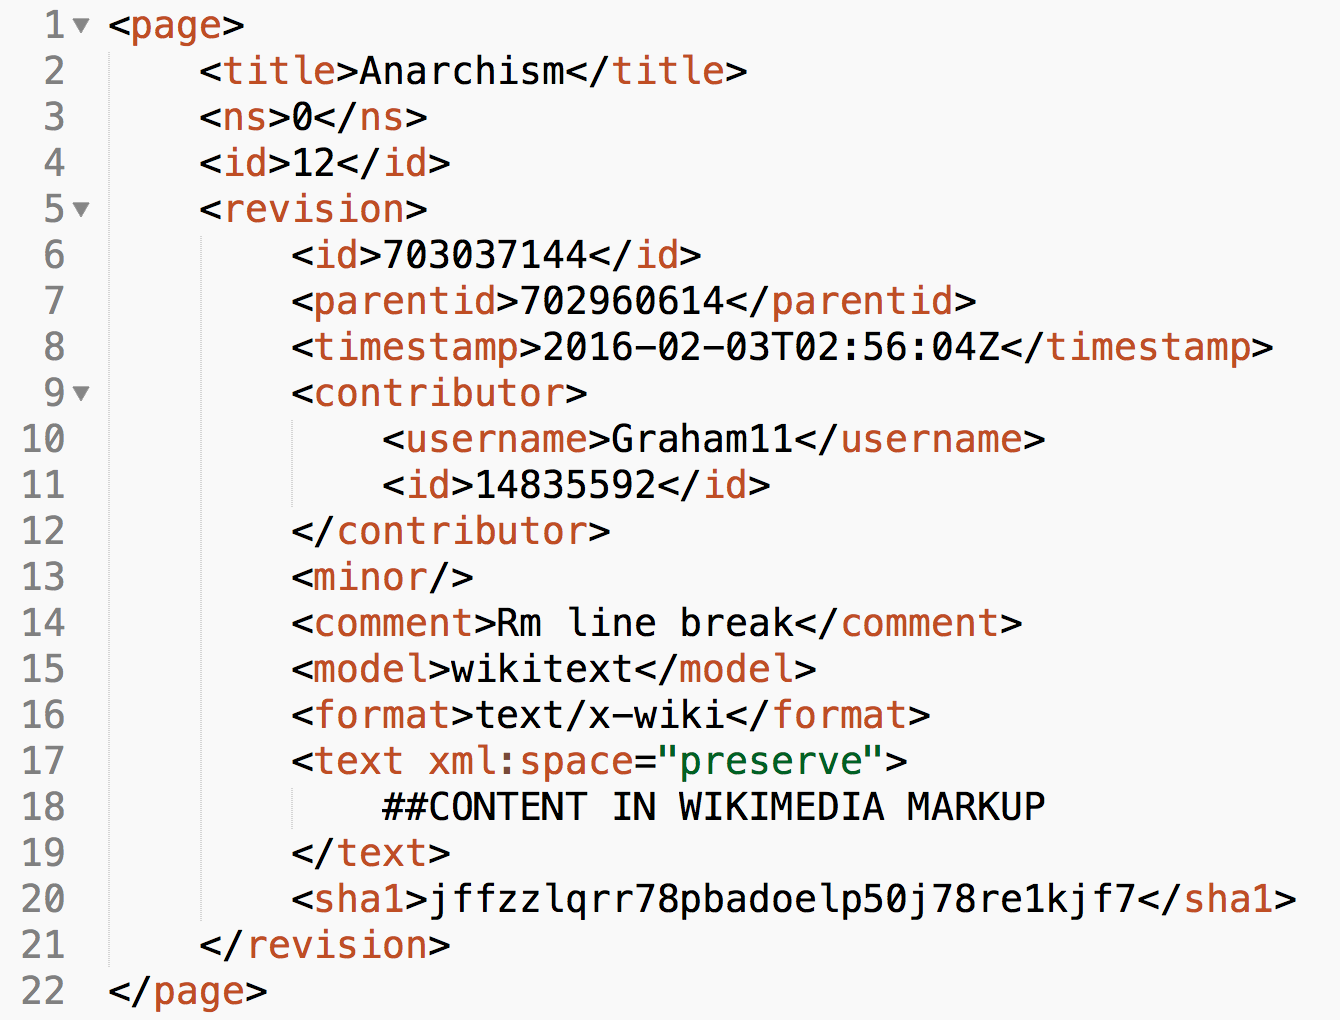
\includegraphics[width=\textwidth]{XMLPage}
\label{fig:xml}
\end{figure}

The source data that is fed into the beginning of the pipeline is on the XML format. \ref{fig:xml} shows how the XML is structured. The file is composed of page elements at the top level with the page tag. Each page element represents an article in Wikipedia. the page has several sub elements, but the most interesting element, is the one with the revision tag. Wikipedia saves several revisions of a page, but in the XML dump used only the newest one is included. It is inside this element that we find the article's content in the form of Wiki markup.


\subsubsection{XML parsing}
In our project the JavaScript class \texttt{XMLParser.js} handles the parsing of XML. It detects where an article in the XML document starts and where it ends, then proceeds to send the content to \texttt{index.js}. The document is read as a stream, which gives the advantage of only keeping a small bit of the document in memory. The library \textit{sax}\footnote{\url{https://www.npmjs.com/package/sax}} is used to read the document as a stream. Sax then uses events for indicating what in the document it is currently reading. Our project listens to the events for a open tag, close tag and content. By saving the state of which element Sax currently is inside we extract text, title, id and timestamp from an articles contents. When we detect the end of an article element, the data extracted is passed to \texttt{index.js}.


\subsection{Data retrieval}


%%Parsing XML into relevant data in JSON
\subsubsection{Wiki markup}
\begin{figure}[h]
\caption{A short outline from an article's wiki markup, with important aspects highlighted and marked. }
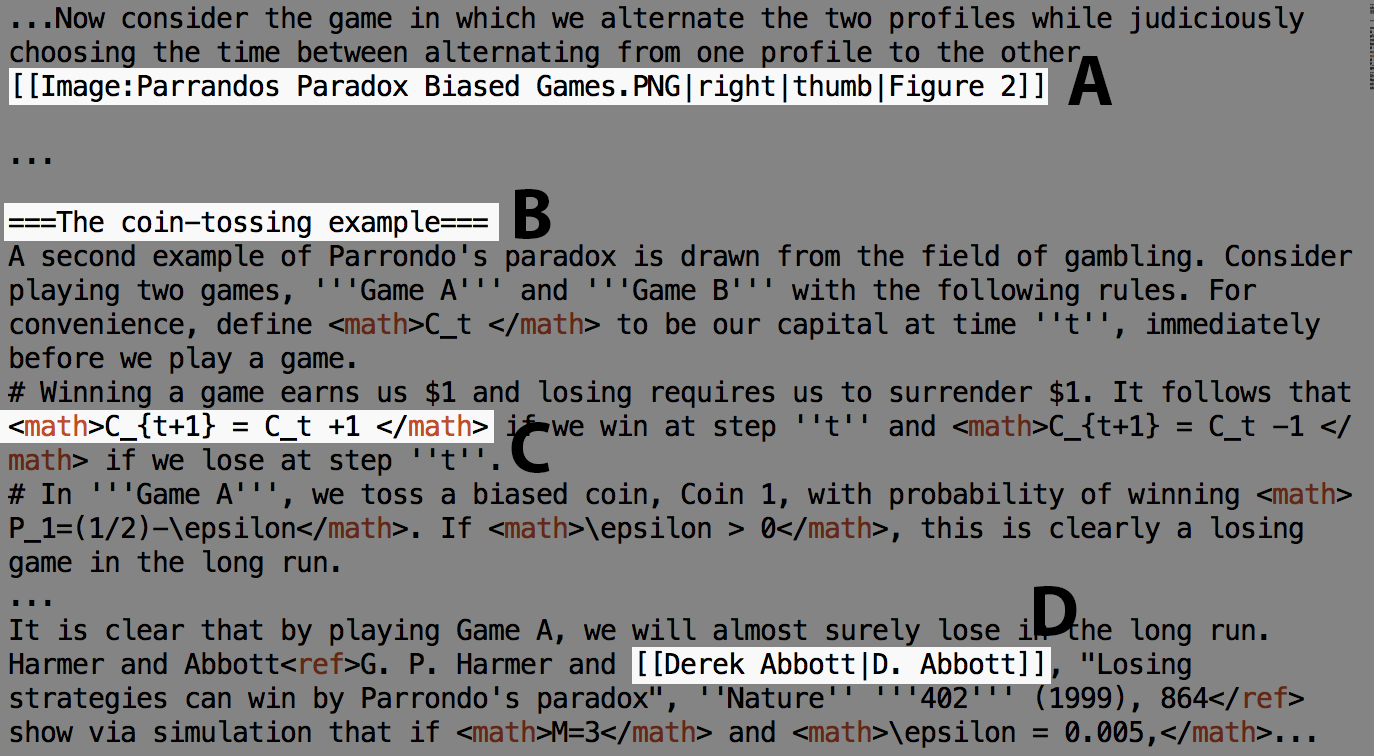
\includegraphics[width=\textwidth]{wiki_markup_marked}
\label{fig:wiki_markup}
\end{figure}

When extracting data from the Wikipedia articles, the articles markup is processed. The markup is called \textit{wiki markup}. Figure \ref{fig:wiki_markup} points out some important aspects of the markup language, for a complete guide, Wikipedia has its own help page\footnote{Help:wiki markup - \url{https://en.wikipedia.org/wiki/Help:Wiki_markup}}. Mark \texttt{A} shows how to refer to an image or other graphic. The first piece of information is about where to find it in Wikipedia's database, while the rest is visual. Mark \texttt{B} is the most important markup when dividing the article into sections. The equal signs at each side indicates that it is a header for a section. The number of equal signs range from one to six. One is the Article title, two is section, three is subsection and so on. By using the hierarchy we can both separate out sections from each other and find each sections parent section.

The markup by Mark \texttt{C} is used for special formatting between the tags. In the case of figure \ref{fig:wiki_markup} mathematical expressions are shown. Syntax for code is another tag that is often included in examples, it is marked like this, \texttt{<source lang="java">}, where the value of \texttt{lang} is the programming language. Mark \texttt{D} shows how one Wikipedia article refers to another. When parsing the sections, all these references are stored. These references are later used for finding relations and relevance between two articles. The words right of the pipe is the reference name, while the ones on the left is the name of the article that are linked to. 




\subsubsection{Markup parsing}
Each article sent to \texttt{index.js} from \texttt{XMLParser.js} is assessed on whether it contains examples or not. Articles who does not contain any examples, are discarded completely from the final collection. In order to assess the articles, the markup is parsed into objects. This is the task of \texttt{MarkupParser.js}. The parser uses several steps to extract the desired information from the markup. The first steps parses the entire article's markup. The result of the first step is objects for each section, including the introduction. The sections contain a header, what level they belong to in the section hierarchy and the content of the section. 

The next step iterates through the list of sections to determine if some of them is an example. Sections which are not an example is discarded. If no examples are found, the whole article is discarded at this point. References to other articles and categories are then extracted from the markup. The data is finally inserted into the database pictured in figure \ref{fig:db_diagram}.



\subsection{Data structuring}

%%Inserting the JSON into an sql database
\subsubsection{Database}

\begin{figure}[h] 
\caption{A simple overview of the database tables and their attributes}
\includegraphics[width=\textwidth]{db_diagram}
\label{fig:db_diagram}
\end{figure}

%% TODO forklare tabellene bedre. Hva de forskjellige termene er i den faktiske wikipedia

Section \ref{custom-pipeline} explains that the source data is fed into the pipeline as a snapshot of Wikipedia at a particular time. The size of the source data is an approximately 50 GB XML-document. Most of this data is not interesting in this project. Therefor the parser excludes most of it before it is structured in the SQL database. 

Figure \ref{fig:db_diagram} displays the tables of the database and the relations between them. If a relevant article is discovered, it is inserted into the \textit{pages} table. The article is found relevant because it contains one or more sections with an example. These sections are then stored in the database with their relation to the article. The categories of the article is also kept, because it will be helpful regarding searching among examples in the finished index.  

The database acts a temporary buffer for the data going into the index. Having a buffer separates the parsing, from the building of the index. Therewith changes made in the parsing, will not affect the rest, so the database acts as a interface between the parser and the indexer. The data is stored on disk, so also the point in time when the programs are executed can happen independently.

This is preferred since the parsing is a very time consuming process, and having it structured in SQL with its meta data helps with showing how successful the parsing was. Some of the meta data is also irrelevant for the index, so only keeping it in the database is makes the end result less complex.


\subsection{Indexing data}
A java program queries the database for all the sections. The relations and data from the other tables are incorporated into the section. Now the section is an object with all the data needed to independently represent an example.

Before the examples are inserted into the index, the index is created with the Elasticsearch java API\footnote{\url{https://www.elastic.co/guide/en/elasticsearch/client/java-api/current/index.html}}. Our project uses the default settings, so only the cluster named is needed to be defined beforehand, the rest happens automatically by Elasticsearch. Lastly a mapping for the example object is passed to Elasticsearch. Figure \ref{fig:es_mapping} shows the mapping passed. It defines all the fields with its types. The mapping sets \textit{categories} to \texttt{not\_analyzed}, so it will match the exact category names.

\begin{figure}[h] 
\caption{Mapping used to define an example in Elasticsearch}
\centering
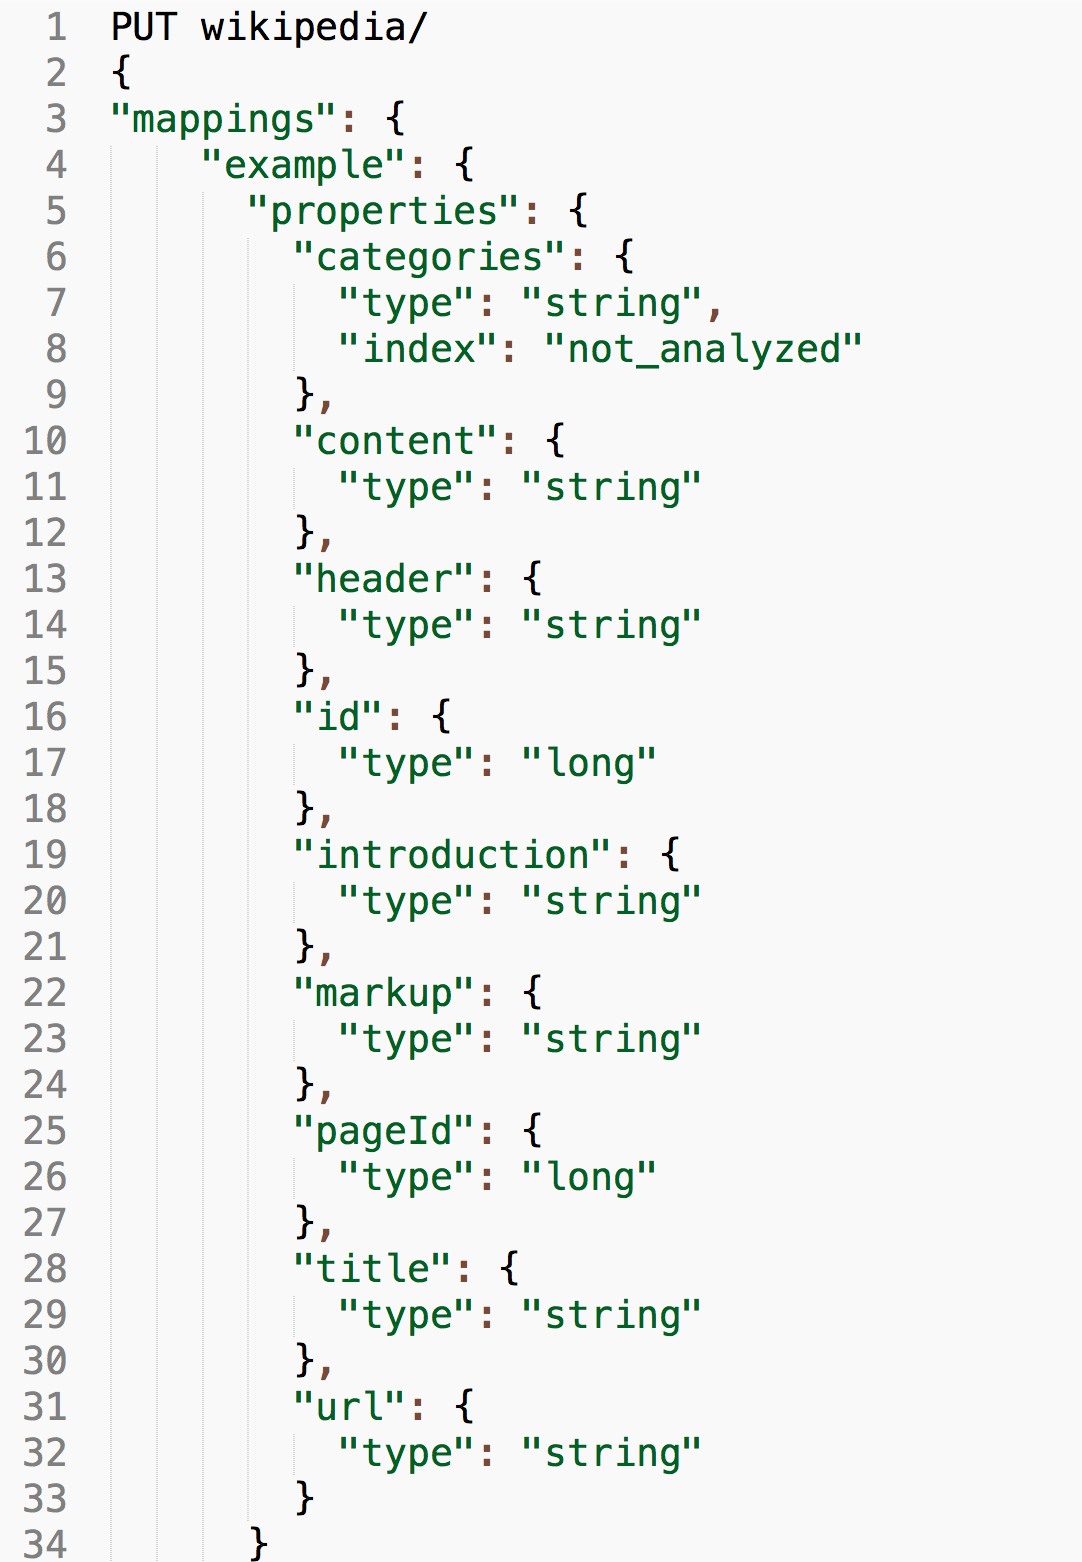
\includegraphics[scale=0.5]{es_mapping}
\label{fig:es_mapping}
\end{figure}

To put each example into the index, they first have to be converted to JSON. A simple methods maps all fields over to an equivalent attributes. Attributes in JSON is key-value pairs, so a key name and the field's value is used. The Java API sends each example to Elasticsearch as a document on the JSON format, which then indexes it.

\subsection{Search interface}


\cleardoublepage